\paragraph{La classe ProtocolCANdroid}


\begin{minipage}
    {\linewidth}
    \centering
    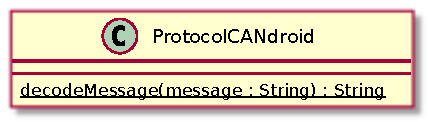
\includegraphics[width=0.50\linewidth]{../schemas/Conception_detaillee/classe_protocolCANdroid.pdf}
    \captionof{figure}{Diagramme de classe de ProtocolCANdroid}
\end{minipage}
\subparagraph{Philosophie de conception \newline} 

\medspace

La classe ProtocolCANdroid a pour rôle de décoder le message reçu par le programme {\nomLogiciel}. 

\subparagraph{Description structurelle \newline}

\medspace

\textbf{Attributs :}

N.A.

\textbf{Services offerts :}

\begin{itemize}
    \item \textbf{decodeMessage(message : String) : String} --- Opération qui permet le décodage du message reçu. L'application {\nomApplication} reçoit \textasciitilde{}frame\#id\$size@message, le décodage permet de retourner \#id\$size@message au dispatcher. 
\end{itemize}

